\begin{frame}
  \frametitle{统计学 | “天书”}
  \begin{figure}
    \centering
    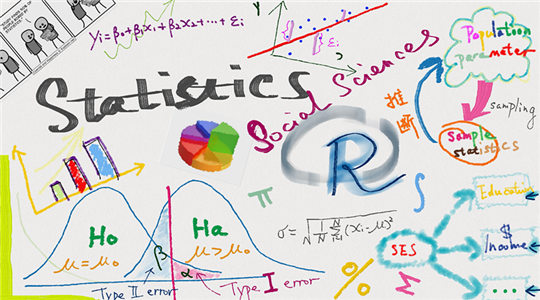
\includegraphics[width=0.55\textwidth]{c0.stats.02.jpg}\\
    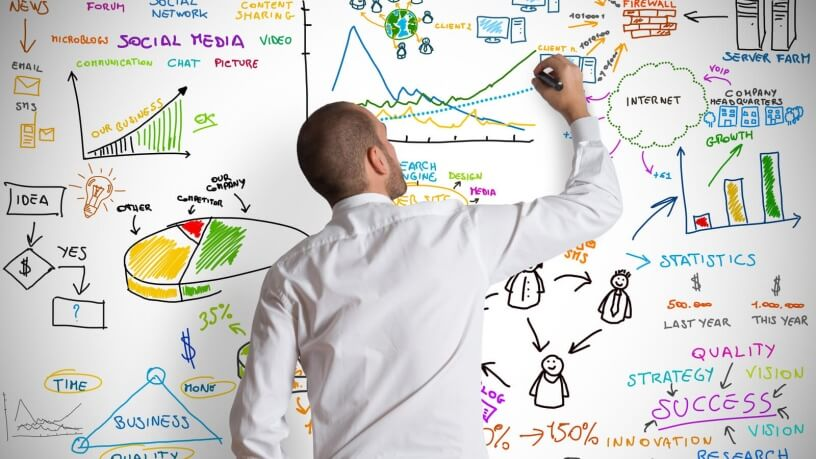
\includegraphics[width=0.55\textwidth]{c0.stats.01.jpg}
  \end{figure}
\end{frame}

\begin{frame}
  \frametitle{统计学 | “谈虎色变”}
  \begin{figure}
    \centering
    \visible<1->{
\includegraphics[width=0.34\textwidth]{c0.stats.03.jpg}}
    \visible<2->{
\includegraphics[width=0.34\textwidth]{c0.stats.04.jpg}}
    \visible<3->{
\includegraphics[width=0.3\textwidth]{c0.stats.05.jpg}}
  \end{figure}
\end{frame}

\begin{frame}[fragile]
  \frametitle{统计学 | 日用而不知}
  \begin{block}{统计无处不在}
    \begin{itemize}
      \item 耶鲁毕业生平均年收入25111美元 
      \item 普通美国人每天刷牙1.02次
      \item 钢铁公司职工平均周收入攀升了107\%
      \item 自从使用了多斯克牌牙膏,我们的蛀牙减少了23\%
      \item 低于智商平均数100的小孩智力有问题
      \item 一个四口之家的平均总收入为5004美元
      \item ……
    \end{itemize}
  \end{block}
  \pause
  \begin{block}{统计充斥着整个社会、各个行业}
    社会经济、商业状况、民意调查、学术报道……
  \end{block}
\end{frame}

\begin{frame}
  \frametitle{统计学 | 日用而不知 | 城市快报20170419(1/4)}
  \begin{figure}
    \centering
    
\includegraphics[width=0.3\textwidth]{c0.tjkb.01.jpg}\quad
    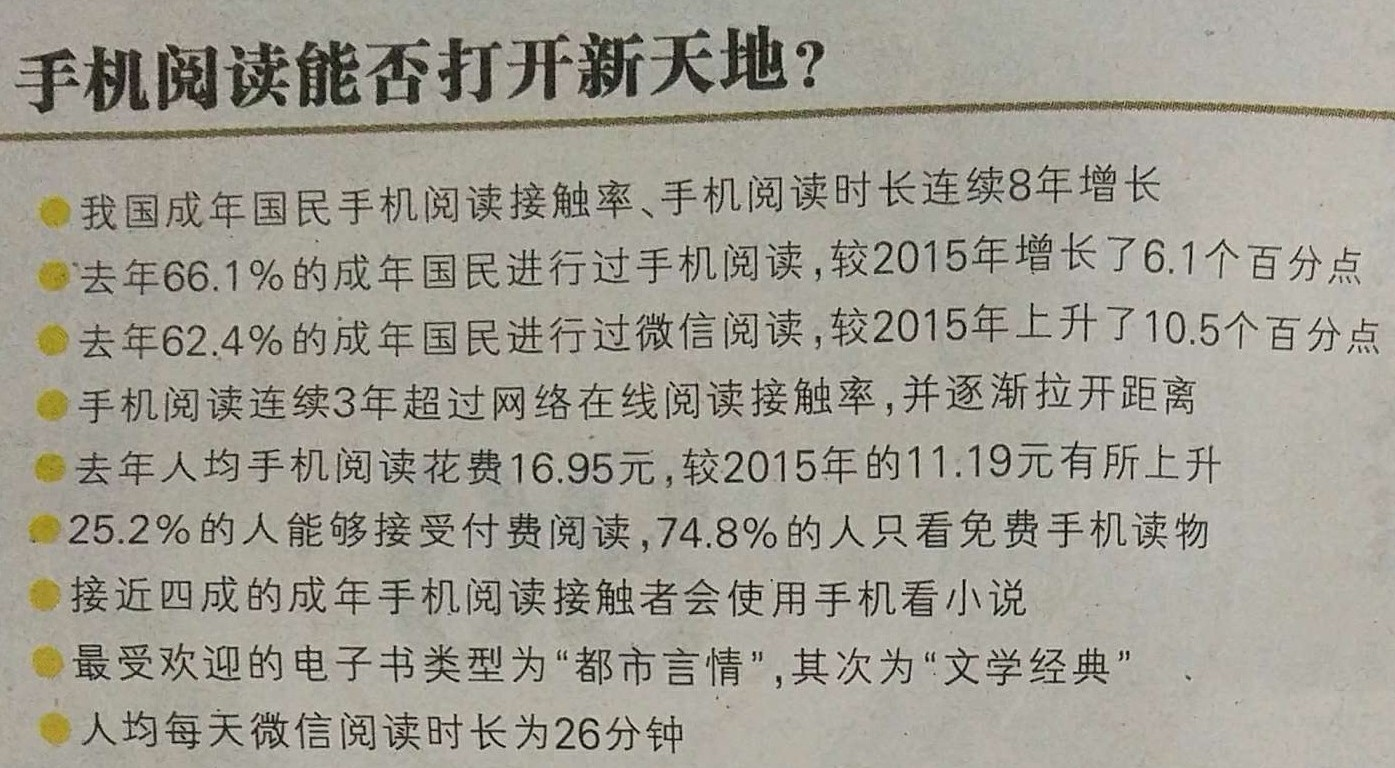
\includegraphics[width=0.51\textwidth]{c0.tjkb.02.01.jpg}\\
    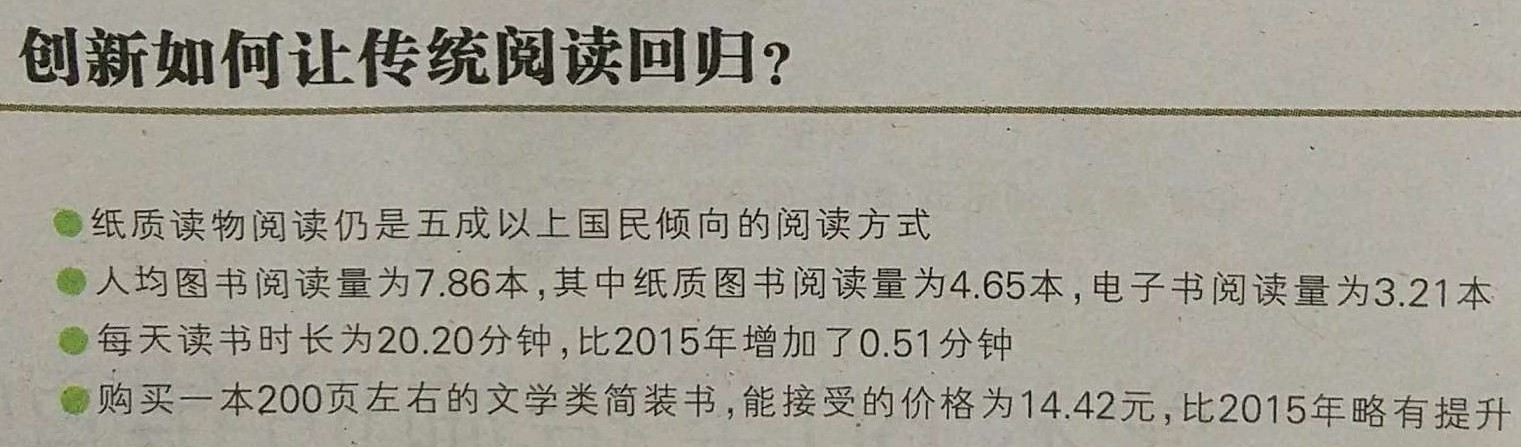
\includegraphics[width=0.45\textwidth]{c0.tjkb.02.02.jpg}\quad
    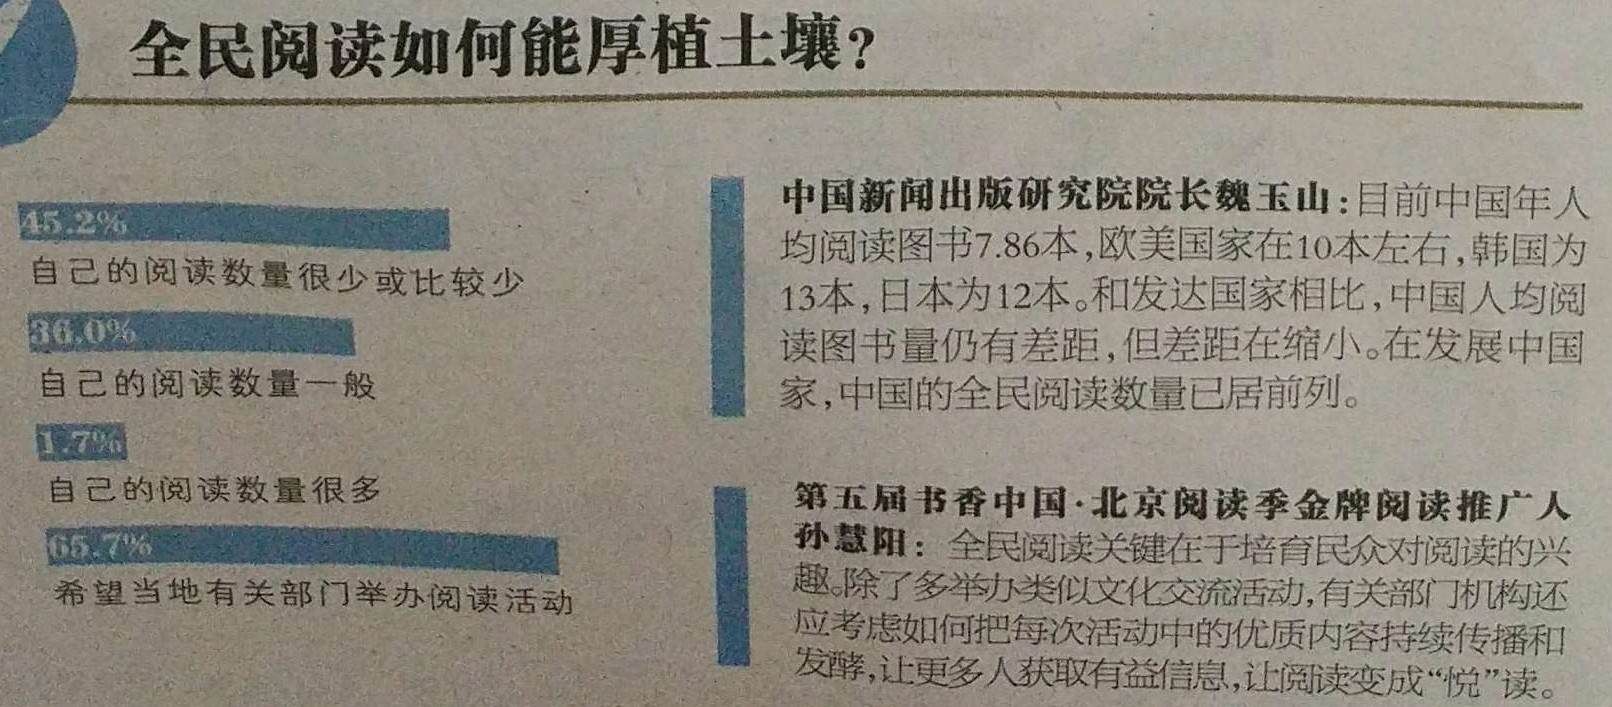
\includegraphics[width=0.5\textwidth]{c0.tjkb.02.03.jpg}\\
  \end{figure}
\end{frame}

\begin{frame}
  \frametitle{统计学 | 日用而不知 | 城市快报20170419(2/4)}
  \begin{figure}
    \centering
    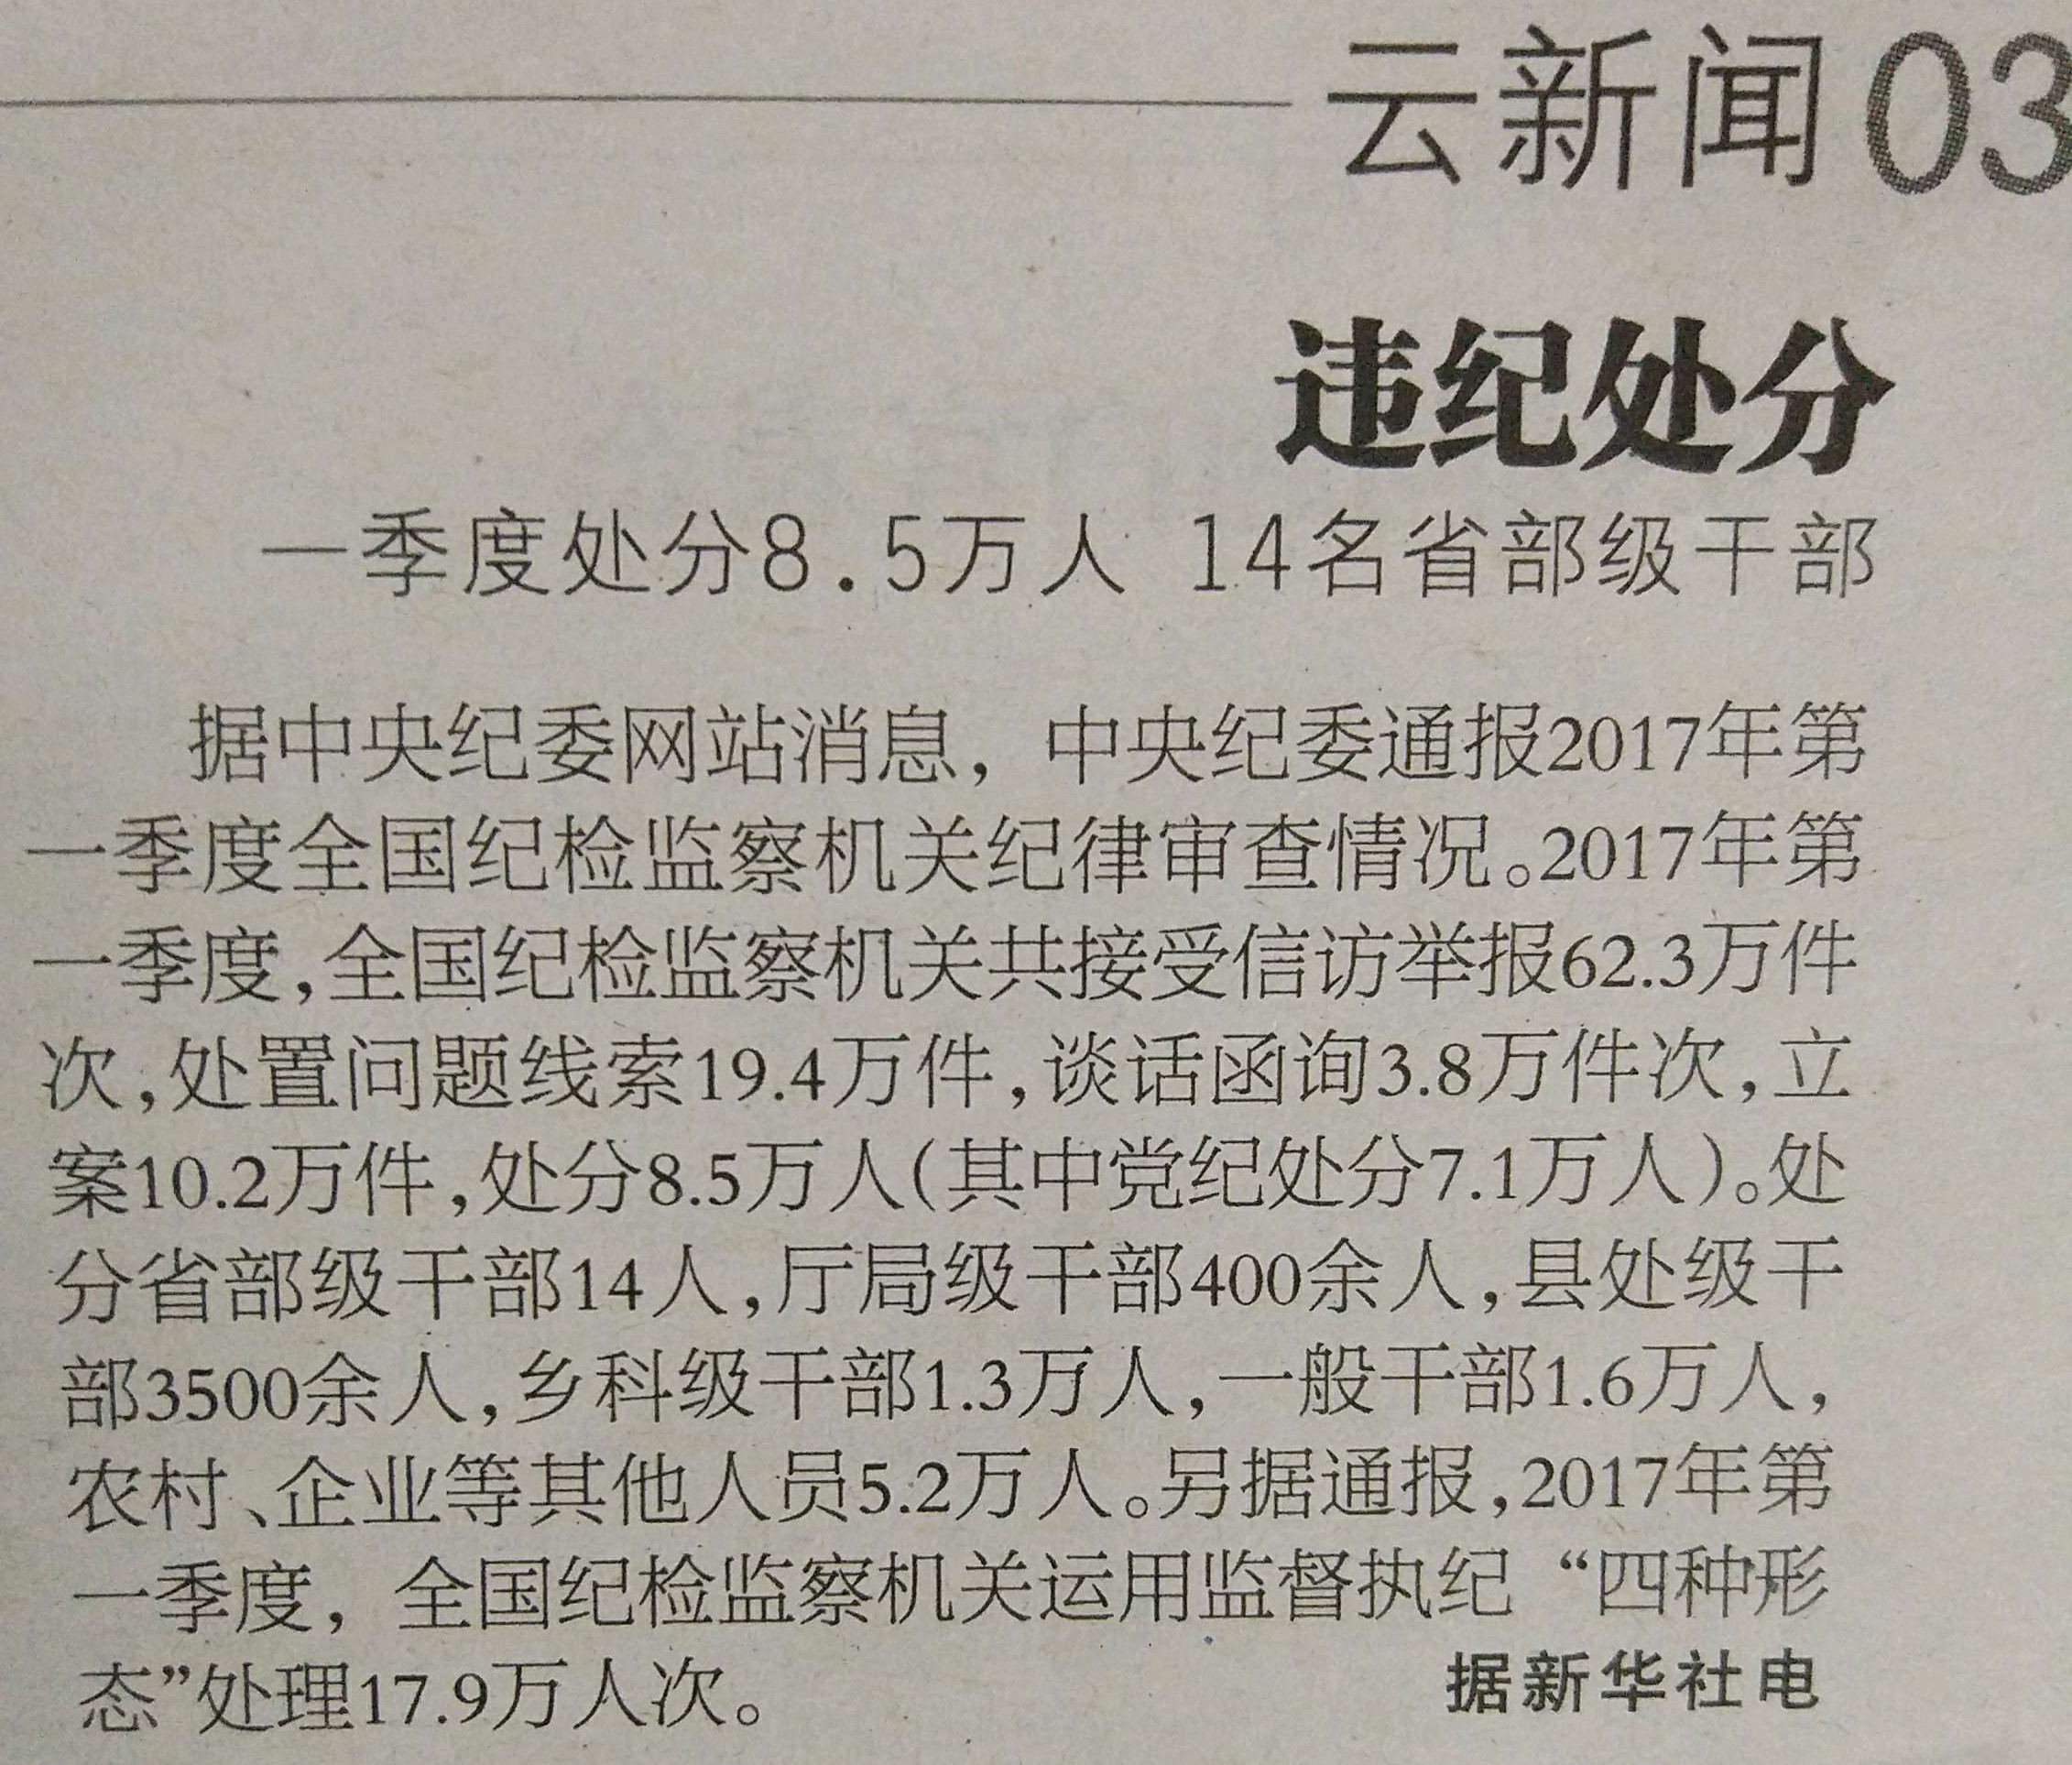
\includegraphics[width=0.48\textwidth]{c0.tjkb.03.jpg}\quad
    
\includegraphics[width=0.47\textwidth]{c0.tjkb.04.jpg}
  \end{figure}
\end{frame}

\begin{frame}
  \frametitle{统计学 | 日用而不知 | 城市快报20170419(3/4)}
  \begin{figure}
    \centering
    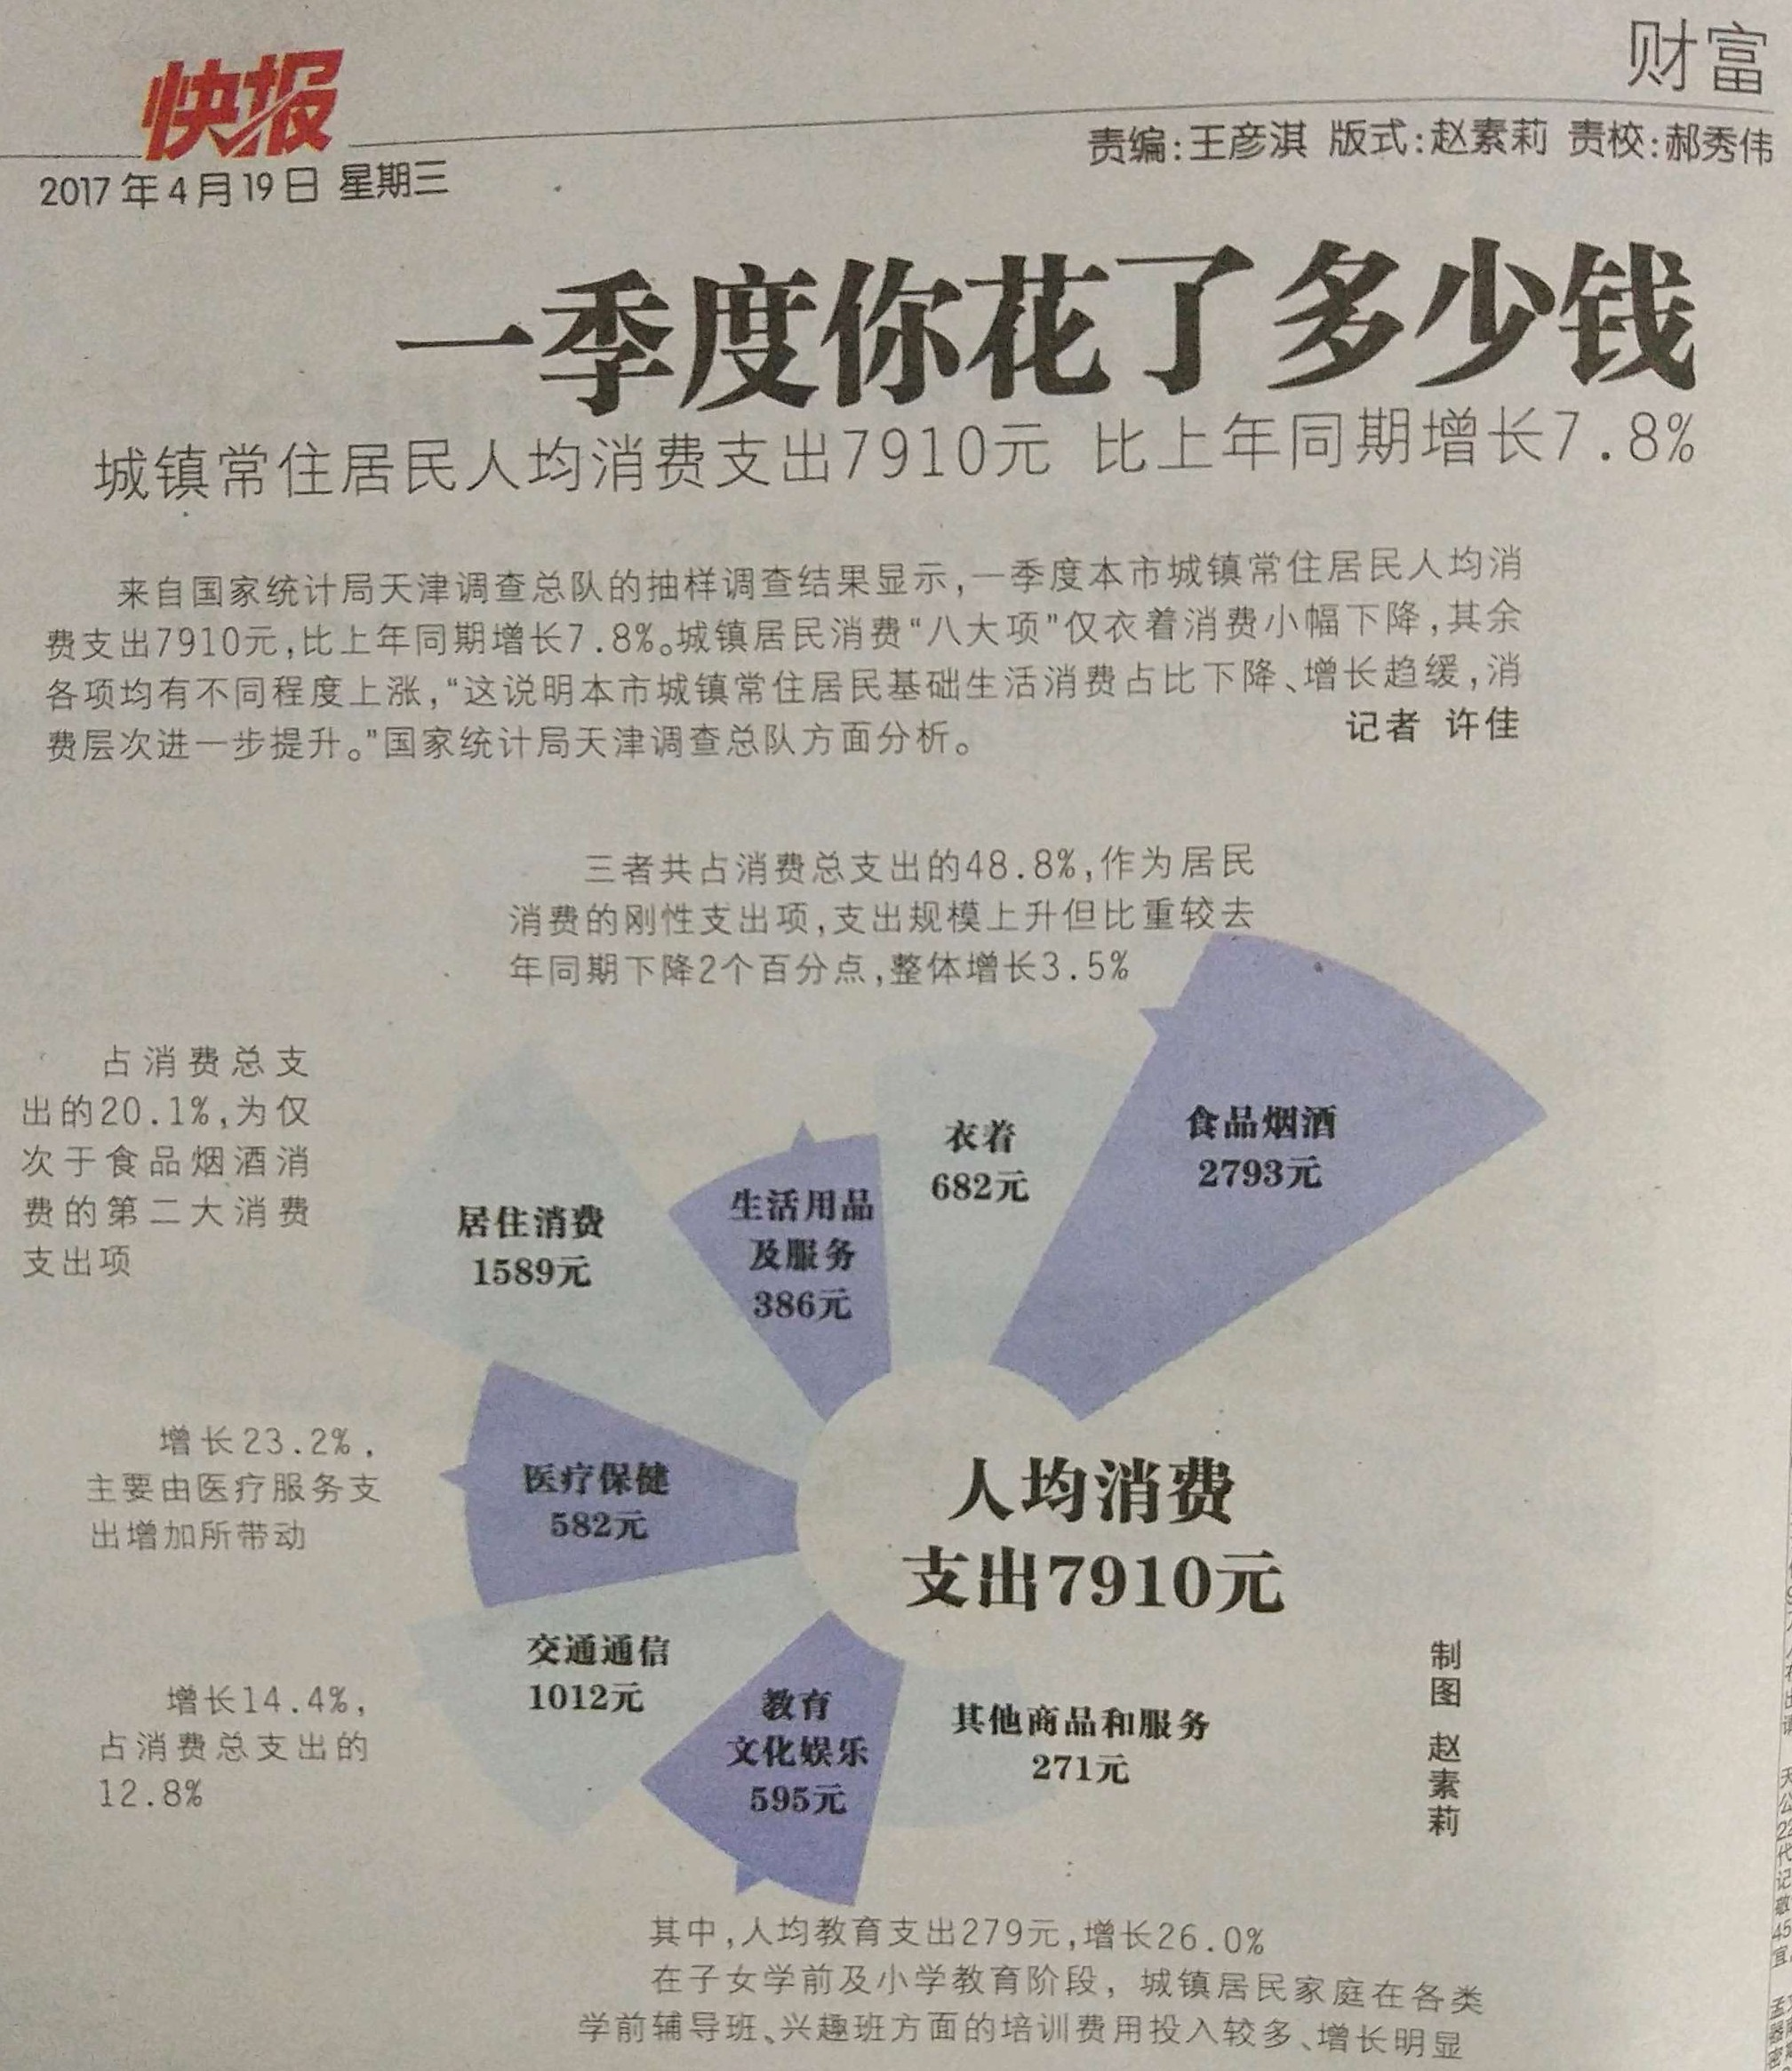
\includegraphics[width=0.45\textwidth]{c0.tjkb.05.jpg}\quad
    
\includegraphics[width=0.5\textwidth]{c0.tjkb.06.jpg}
  \end{figure}
\end{frame}

\begin{frame}
  \frametitle{统计学 | 日用而不知 | 城市快报20170419(4/4)}
  \begin{figure}
    \centering
    
\includegraphics[width=0.48\textwidth]{c0.tjkb.07.jpg}\quad
    
\includegraphics[width=0.48\textwidth]{c0.tjkb.08.jpg}
  \end{figure}
\end{frame}

\begin{frame}
  \frametitle{统计学 | 日用 $\rightarrow$ 滥用 $\rightarrow$ 陷阱}
  \begin{block}{眼见为实?}
    \begin{itemize}
      \item 虽然经验告诉我们“眼见为实”,但眼睛告诉我们的“真相”或许隐藏了部分事实,或许夸大了事实。
      \item 如果作者不能正确理解并恰当地使用统计语言,而读者又并不能真正了解这些术语的含义,那么,统计结果只能是废话一堆。
    \end{itemize}
  \end{block}
  \pause
  \begin{block}{陷阱随处可见}
    \begin{itemize}
      \item 统计这种神秘的语言,在一个靠事实说话的社会里是如此地吸引眼球,但有时它却被人利用,并成为恶意夸大或简化事实、迷惑他人的工具。
      \item 大量的统计数据、统计资料由于主、客观的原因被滥用,很难起到描述事实、传递信息的作用。相反,还往往对读者形成误导。
      \item 使我们陷入麻烦的通常并非我们不知道的事情,而是那些我们知道得不确切的事情。
    \end{itemize}
  \end{block}
\end{frame}

\begin{frame}
  \frametitle{统计学 | 说谎的统计数字}
  \begin{block}{质疑“平均工资”}
    \begin{itemize}
      \item 2004年,广州市职工平均工资为28237元。
      \item 市民普遍反映年工资收入基本达不到这个水平,有的甚至相距甚远。
    \end{itemize}
  \end{block}
  \pause \pause \pause \pause
  \begin{block}{“谎言”的背后}
    \begin{itemize}
      \item 职工统计中有七类人员没有列入范围,而这部分人正属于收入较低的群体。
      \item 当数据的分布呈现正偏态时,均值往往偏离一般水平,并且高于一般水平。
    \end{itemize}
  \end{block}
\end{frame}

\begin{frame}[fragile]
  \frametitle{课程主旨}
  \begin{block}{统计 vs. 谎言 vs. 技能}
    \begin{itemize}
      \item 有3种谎言:谎言、糟糕透顶的谎言和统计资料。
      \item 对于追求效率的公民而言,统计思维总有一天会和读写能力一样必要。
      \item 骗子对于行骗的技巧早已胸有成竹,而诚实的人出于自卫也应该掌握它。
    \end{itemize}
  \end{block}
  \pause
  \vspace{-0.5em}
  \begin{figure}
    \centering
    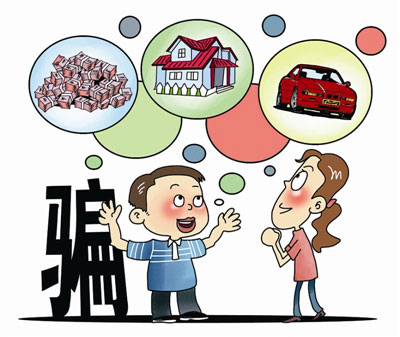
\includegraphics[width=0.35\textwidth]{c0.object.01.jpg}
    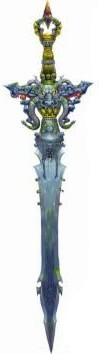
\includegraphics[width=0.1\textwidth]{c0.object.03.jpg}
    
\includegraphics[width=0.3\textwidth]{c0.object.02.jpg}
  \end{figure}
\end{frame}

\begin{frame}
  \frametitle{课程主旨}
  \begin{block}{对数据的态度——怀疑+思考}
    如果一个人以种种肯定的立论开始,他必将终止于各种怀疑;但如果他愿意抱着怀疑的态度开始,那么他必将获得肯定的结论。
  \end{block}
  \pause
  \begin{block}{练就看穿统计资料的“火眼金睛”}
    对统计资料应该提出五个问题:
    \begin{enumerate}
      \item 谁说的
      \item 如何知道的
      \item 是否遗漏了什么
      \item 是否偷换了概念
      \item 资料是否有意义
    \end{enumerate}
  \end{block}
\end{frame}

\begin{frame}
  \frametitle{参考教材}
  \begin{figure}
    \centering
    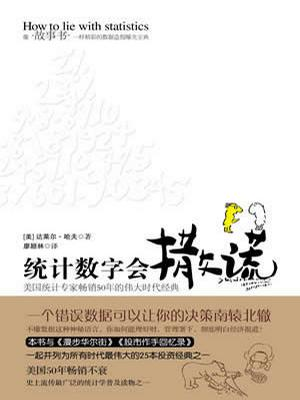
\includegraphics[width=2.8cm]{c0.book.01.jpg}\qquad
    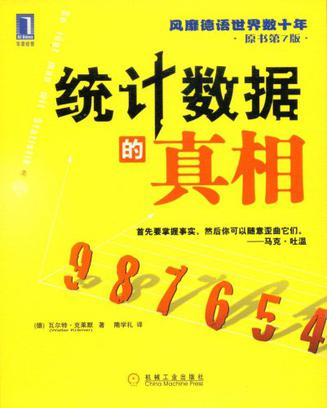
\includegraphics[width=2.8cm]{c0.book.02.jpg}\\
    
\includegraphics[width=2.6cm]{c0.book.03.jpg}\qquad
    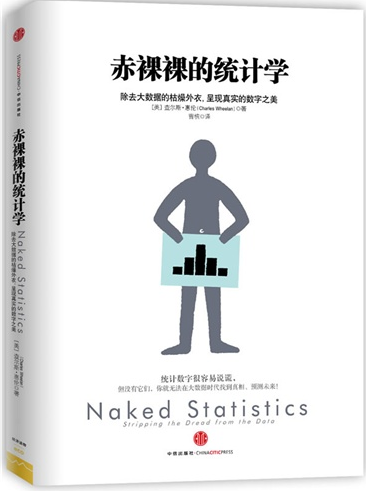
\includegraphics[width=3cm]{c0.book.04.png}
  \end{figure}
\end{frame}

\begin{frame}
  \frametitle{课外读物}
    \begin{block}{统计学与数据分析}
      \begin{multicols}{2}
      \begin{itemize}
         \item 《统计会犯错》
         \item 《生活中的概率趣事》
         \item 《改变世界的134个概率统计故事》
         \item 《介绍丛书:统计学》
         \item 《漫画玩转统计学》
         \item 《漫画统计学》
         \item 《白话统计学》
         \item 《爱上统计学》
         \item 《统计学的世界》
         \item 《从零开始读懂统计学》
         \item 《你一定爱读的极简统计学》
         \item 《深入浅出统计学》
         \item 《深入浅出数据分析》
         \item 《菜鸟侦探挑战数据分析》
         \item 《妙趣横生的统计学》
         \item 《有趣的统计》
         \item 《统计学漫话》
         \item 《统计学七支柱》
        \end{itemize}
      \end{multicols}
    \end{block}
\end{frame}

\begin{frame}
  \frametitle{微信公众号 | 狗熊会}
  \begin{figure}
    \centering
    
\includegraphics[width=0.6\textwidth]{c0.wx.gxh.jpg}
  \end{figure}
\end{frame}

\begin{frame}
  \frametitle{微信公众号 | 统计之都}
  \begin{figure}
    \centering
    
\includegraphics[width=0.6\textwidth]{c0.wx.tjzd.jpg}
  \end{figure}
\end{frame}

\begin{frame}
  \frametitle{微信公众号 | 雪晴数据网}
  \begin{figure}
    \centering
    
\includegraphics[width=0.6\textwidth]{c0.wx.xqsjw.jpg}
  \end{figure}
\end{frame}
\begin{frame}
  \frametitle{微信公众号 | 复旦大数据}
  \begin{figure}
    \centering
    
\includegraphics[width=0.6\textwidth]{c0.wx.fddsj.jpg}
  \end{figure}
\end{frame}

\begin{frame}
  \frametitle{授课资料}
  \begin{figure}
    \centering
    
\includegraphics[width=0.55\textwidth]{qr.png}
  \end{figure}
  \begin{center}
    \href{https://github.com/Yixf-Education/course_Statistics_Story}{https://github.com/Yixf-Education/course\_Statistics\_Story}
  \end{center}
\end{frame}

% \begin{frame}
%   \frametitle{短片视频}
%   \begin{figure}
%     \centering
%     
\includegraphics[width=0.55\textwidth]{c0.short.movie.png}
%   \end{figure}
%   \begin{center}
%     \href{http://www.tudou.com/listplay/YUwEELLXLoI.html}{http://www.tudou.com/listplay/YUwEELLXLoI.html}
%   \end{center}
% \end{frame}

\begin{frame}
  \frametitle{课程安排}
  \begin{center}
  \alert{前8周,每周三,晚上两节(18:00-20:00),西楼506}\\
  \vspace{0.2cm}
  \end{center}
  \begin{block}{授课内容}
    \begin{itemize}
      \item 抽样、均值、误差、趋势、图形、相关、技巧……
      \item 剖析经典的故事实例,介绍基本的统计思想
      \item 图说天下,谈天说地,评古论今
    \end{itemize}
  \end{block}
\end{frame}

\begin{frame}
  \frametitle{\alert{考核方式}}
  \begin{block}{考勤}
    \begin{itemize}
      \item 不点名,但随机提问
      \item 缺勤0次——优秀(及以下)
      \item 缺勤1次——良好(及以下)
      \item 缺勤2次——及格(及以下)
      \item \alert{缺勤3次——不及格}
    \end{itemize}
  \end{block}
  \pause
  \begin{block}{报告}
    \begin{itemize}
      \item 内容:自己关于某个(错误)统计数字/图形/资料/报道的思考
      \item 要求:电子版,~500字(一页纸),含信息来源、资料分析等;\alert{抄袭——不及格}
      \item 提交:yixfbio@gmail.com,课程名-学号-姓名-共享/保密.doc
      \item 示例:在Word里面撰写 $\rightarrow$ 重命名为“故事中的统计学-201600-张三-共享.doc” $\rightarrow$ 发送邮件 $\rightarrow$ 等待回复
    \end{itemize}
  \end{block}
\end{frame}

